% This is "sig-alternate.tex" V2.0 May 2012
% This file should be compiled with V2.5 of "sig-alternate.cls" May 2012
%
% This example file demonstrates the use of the 'sig-alternate.cls'
% V2.5 LaTeX2e document class file. It is for those submitting
% articles to ACM Conference Proceedings WHO DO NOT WISH TO
% STRICTLY ADHERE TO THE SIGS (PUBS-BOARD-ENDORSED) STYLE.
% The 'sig-alternate.cls' file will produce a similar-looking,
% albeit, 'tighter' paper resulting in, invariably, fewer pages.
%
% ----------------------------------------------------------------------------------------------------------------
% This .tex file (and associated .cls V2.5) produces:
%       1) The Permission Statement
%       2) The Conference (location) Info information
%       3) The Copyright Line with ACM data
%       4) NO page numbers
%
% as against the acm_proc_article-sp.cls file which
% DOES NOT produce 1) thru' 3) above.
%
% Using 'sig-alternate.cls' you have control, however, from within
% the source .tex file, over both the CopyrightYear
% (defaulted to 200X) and the ACM Copyright Data
% (defaulted to X-XXXXX-XX-X/XX/XX).
% e.g.
% \CopyrightYear{2007} will cause 2007 to appear in the copyright line.
% \crdata{0-12345-67-8/90/12} will cause 0-12345-67-8/90/12 to appear in the copyright line.
%
% ---------------------------------------------------------------------------------------------------------------
% This .tex source is an example which *does* use
% the .bib file (from which the .bbl file % is produced).
% REMEMBER HOWEVER: After having produced the .bbl file,
% and prior to final submission, you *NEED* to 'insert'
% your .bbl file into your source .tex file so as to provide
% ONE 'self-contained' source file.
%
% ================= IF YOU HAVE QUESTIONS =======================
% Questions regarding the SIGS styles, SIGS policies and
% procedures, Conferences etc. should be sent to
% Adrienne Griscti (griscti@acm.org)
%
% Technical questions _only_ to
% Gerald Murray (murray@hq.acm.org)
% ===============================================================
%
% For tracking purposes - this is V2.0 - May 2012

\documentclass{sig-alternate}

\usepackage{algorithm}
\usepackage{algpseudocode}

\begin{document}
%
% --- Author Metadata here ---
\conferenceinfo{CS 760}{'14, Madison WI, USA}
\CopyrightYear{2014} % Allows default copyright year (20XX) to be over-ridden - IF NEED BE.
%\crdata{0-12345-67-8/90/01}  % Allows default copyright data (0-89791-88-6/97/05) to be over-ridden - IF NEED BE.
% --- End of Author Metadata ---

\title{BoostEM}
\subtitle{A Semi-Supervised Ensemble Method}
%
% You need the command \numberofauthors to handle the 'placement
% and alignment' of the authors beneath the title.
%
% For aesthetic reasons, we recommend 'three authors at a time'
% i.e. three 'name/affiliation blocks' be placed beneath the title.
%
% NOTE: You are NOT restricted in how many 'rows' of
% "name/affiliations" may appear. We just ask that you restrict
% the number of 'columns' to three.
%
% Because of the available 'opening page real-estate'
% we ask you to refrain from putting more than six authors
% (two rows with three columns) beneath the article title.
% More than six makes the first-page appear very cluttered indeed.
%
% Use the \alignauthor commands to handle the names
% and affiliations for an 'aesthetic maximum' of six authors.
% Add names, affiliations, addresses for
% the seventh etc. author(s) as the argument for the
% \additionalauthors command.
% These 'additional authors' will be output/set for you
% without further effort on your part as the last section in
% the body of your article BEFORE References or any Appendices.

\numberofauthors{2} %  in this sample file, there are a *total*
% of EIGHT authors. SIX appear on the 'first-page' (for formatting
% reasons) and the remaining two appear in the \additionalauthors section.
%
\author{
% You can go ahead and credit any number of authors here,
% e.g. one 'row of three' or two rows (consisting of one row of three
% and a second row of one, two or three).
%
% The command \alignauthor (no curly braces needed) should
% precede each author name, affiliation/snail-mail address and
% e-mail address. Additionally, tag each line of
% affiliation/address with \affaddr, and tag the
% e-mail address with \email.
%
% 1st. author
\alignauthor
Zach Welch\\
       \affaddr{UW--Madison}\\
       \email{zwelch@cs.wisc.edu}
% 2nd. author
\alignauthor
Steven Johnson\\
       \affaddr{UW--Madison}\\
       \email{sjj@cs.wisc.edu}
}
\date{May 12, 2014}
% Just remember to make sure that the TOTAL number of authors
% is the number that will appear on the first page PLUS the
% number that will appear in the \additionalauthors section.

\maketitle
\begin{abstract}
We introduce BoostEM, a semi-supervised learning algorithm which combines the benefits of using an ensemble method like Boosting with the benefits of using unlabeled data.  BoostEM is intended for use in learning settings with an abundance of unlabeled data, and outperforms the traditional AdaBoost algorithm and learning with fractional data from using Expectation Maximization across a variety of base learners and data sets.
\end{abstract}

% A category with the (minimum) three required fields
\section{Introduction}

It is well established in Machine Learning that labels are difficult to obtain while unlabeled data are abundant in many situations where we would like to classify new instances. Examples of such situations are labeling x-rays as benign or malignant, tweets as instances of bullying, news articles as interesting to a given reader, or whether a photograph contains a given object. Because of this scarcity of labeled instances, using semi-supervised learning techniques, such as Expectation Maximization, to combine unlabeled and labeled data into an integrated model is a good idea to potentially improve learner accuracy and reduce human labour.

This paper describes the development and evaluation of a semi-supervised learning algorithm, BoostEM, which combines the benefits of an ensemble method like Boosting with the benefits of using unlabeled data. The next section provides an overview of related work on Boosting and Expectation Maximization. This section is followed by the details of the BoostEM algorithm and an experimental evaluation of our implementation. We then present the results of our evaluation and discuss our findings and their implications.

\section{Background}
\subsection{Boost}
\subsection{Expectation Maximization}
Expectation is an iterative algorithm which uses the values of existing,complete data points to compute the maximum likelihood estimate for missing values for other, incomplete data. Expectation Maximization was originally introduced in ~\cite{Dempster77maximumlikelihood} and produces a probabalistic distribution of the possible values of missing data given fully labeled data. In the context of semi-supervised learning, there is a set of labeled input data and a potentially much larger set of unlabeled data and for each unlabeled instance u, EM can provide a probability for each label.  These probabilities can be used as fractional instances of labeled data, making the input training set much bigger and diverse and potentially giving a better approximation of the distribution of labels to the learner. In many cases, performance can be drastically improved by using these fractional counts.

Expectation maximization is a general approach and can be augmented to suite a variety of settings and assumptions.  For instance, in our implementation of BoostEM we assume the data is well modeled by a Gaussian mixture model and the instances have weights associated with them.    

     
\section{Related Work}
\section{BoostEM}
The main insight of BoostEM is observing that Boost and Expectation Maximization both attempt to improve the current iteration's results by using information from the previous iteration; BoostEM simply couples the results of the two algorithms together to improve results.  BoostEM uses a weighted EM algorithm, and these weights are identical to the weights used in the Boost algorithm.  At it's most basic level, BoostEM simply runs a weighted Expectation Maximization on the unlabeled instances, and uses the fractional counts to create a weighted training set for some base learner.  The results of this base learner are then used to update the weights, which are then input to EM in the next iteration.

\begin{algorithm}
\caption{BoostEM}\label{euclid}
\begin{algorithmic}[1]
\Procedure{BoostEM}{$L,U,T$}
\For{$t=1 \dots T$}
\State $P_{t} \gets EM(L,U,Wl,Wu)$
\EndFor
\State \textbf{return} $b$
\EndProcedure
\end{algorithmic}
\end{algorithm}

By using a weighted EM, we can place more emphasis on the instances our learner incorrectly classifies in the Gaussian distribution of instances we assume. Or more correctly, since there is no ground truth to the unlabeled instances, we can penalize every prediction from learner $H$ on unlabeled instance $x$ by $1-p(H(x))$, where $p(\dot)$ is the distribution of labels from EM.  In this way, the learner penalizes unexpected labels (ones with small probability) more than expected ones.

Notice as well that using Expectation Maximization for fractional counts and adaBoost can be recovered from BoostEM by setting certain inputs and parameters.  Setting the number of boosting iterations to 1 is equivalent to EM, while inputting no unlabeled instances reduces to traditional labeled Boosting.    
    
\section{Evaluation}
We implemented the BoostEM algorithm in \textsc{python} and evaluated its accuracy against a number of other algorithms using two learners and a variety of parameter settings  as described below.

\subsection{Data sets}


\subsection{Benchmark Algorithms}

\subsection{Methodology}
STEVE
\subsection{Results}


 \begin{figure}
\centering
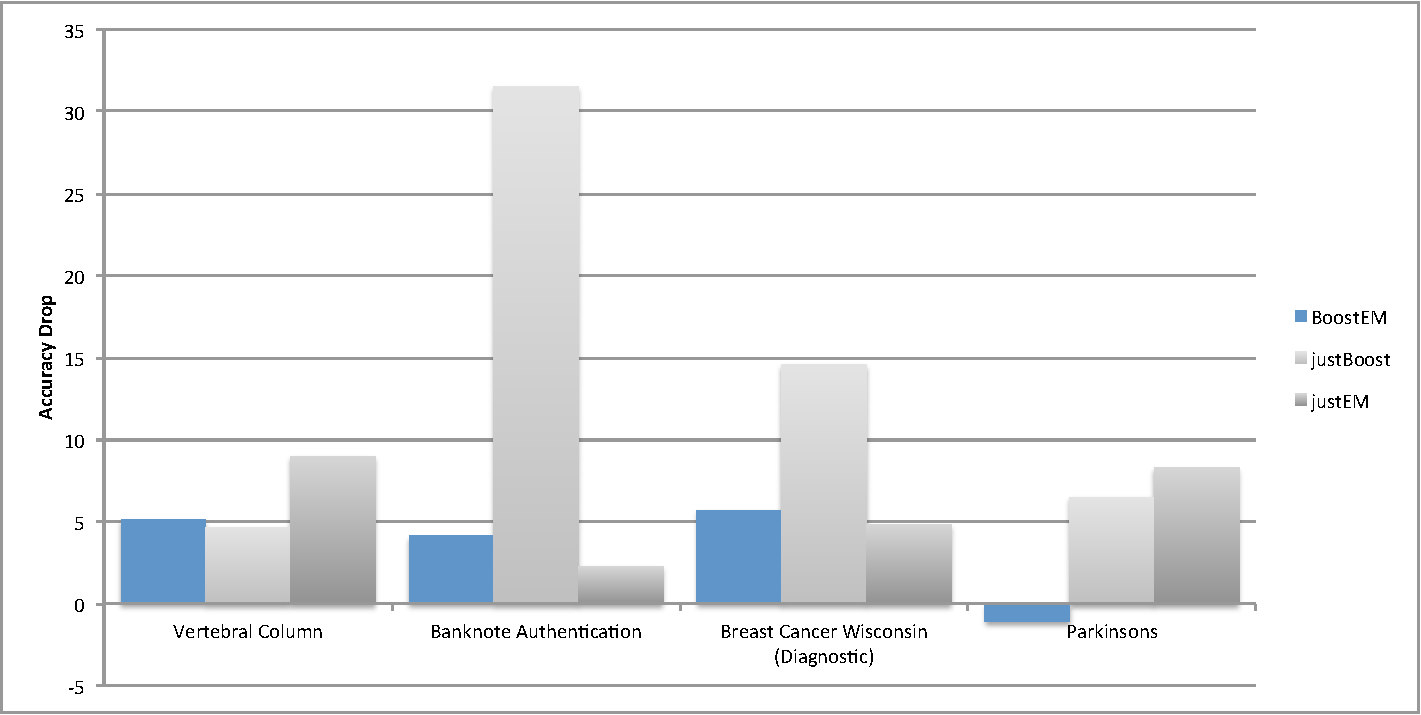
\includegraphics[width=0.5\textwidth]{figures/accDrops.pdf}
\caption{Average decrease in 10 fold cross validation \% accuracy using ID3 from 20\% to 5\% of the data being labeled}
\label{accDrop}
\end{figure}
 
\begin{figure}
\centering
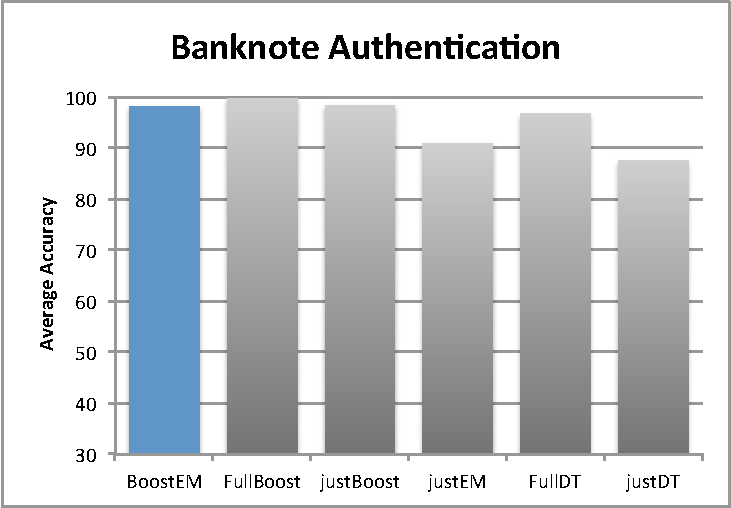
\includegraphics[width=0.3\textwidth]{figures/bankAcc.pdf}
\caption{Average 10 fold cross validation \% accuracy using ID3 on Various algorithms, 20\% labeled data}
\label{bankAcc}
\end{figure}
\begin{figure}
\centering
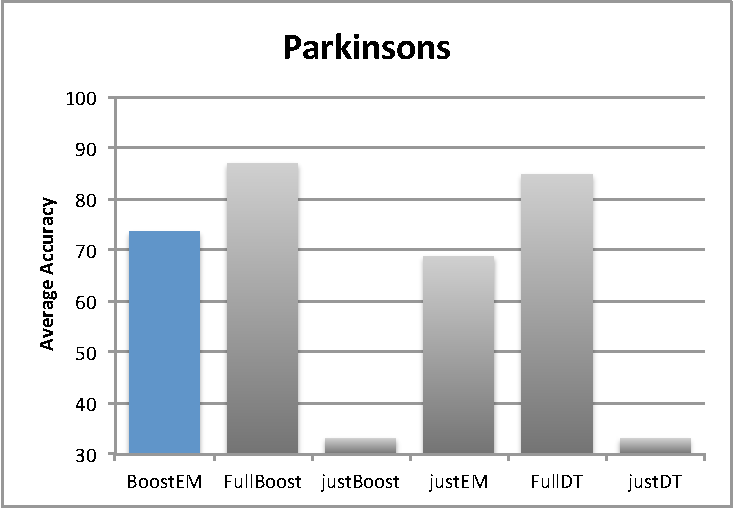
\includegraphics[width=0.3\textwidth]{figures/parkAcc.pdf}
\caption{Average 10 fold cross validation \% accuracy using ID3 on Various algorithms, 20\% labeled data}
\label{parkAcc}
\end{figure}

\begin{figure}
\centering
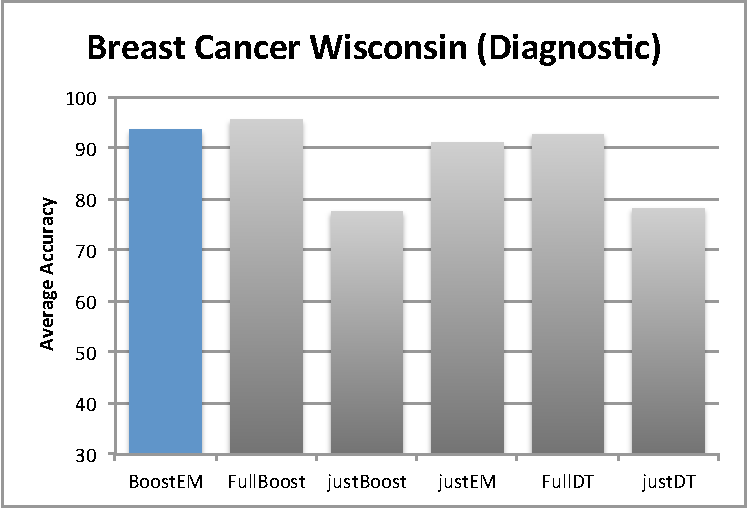
\includegraphics[width=0.3\textwidth]{figures/breaAcc.pdf}
\caption{Average 10 fold cross validation \% accuracy using ID3 on Various algorithms, 20\% labeled data}
\label{breaAcc}
\end{figure}

\begin{figure}
\centering
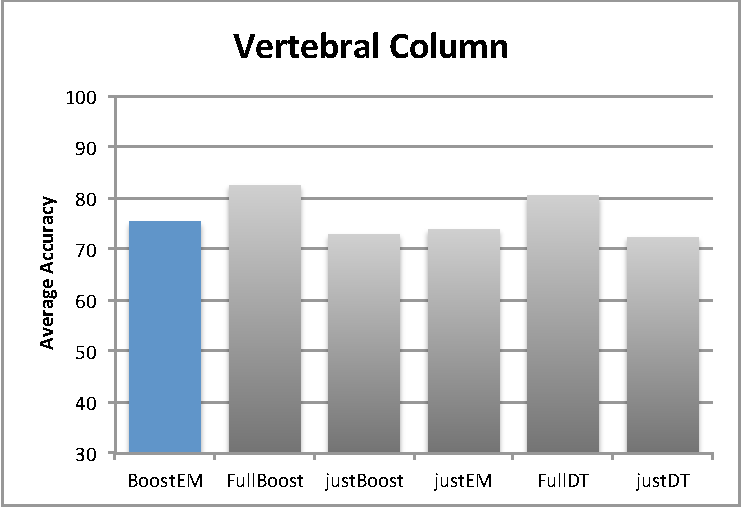
\includegraphics[width=0.3\textwidth]{figures/vertAcc.pdf}
\caption{Average 10 fold cross validation \% accuracy using ID3 on Various algorithms, 20\% labeled data}
\label{vertAcc}
\end{figure}

\begin{figure}
\centering
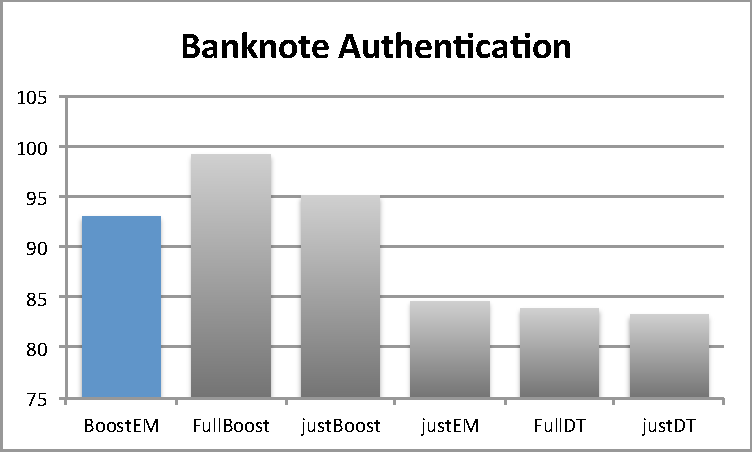
\includegraphics[width=0.3\textwidth]{figures/bankAcc5.pdf}
\caption{Average 10 fold cross validation \% accuracy using Naive Bayes on Various algorithms, 5\% labeled data}
\label{vertAcc}
\end{figure}

\begin{figure}
\centering
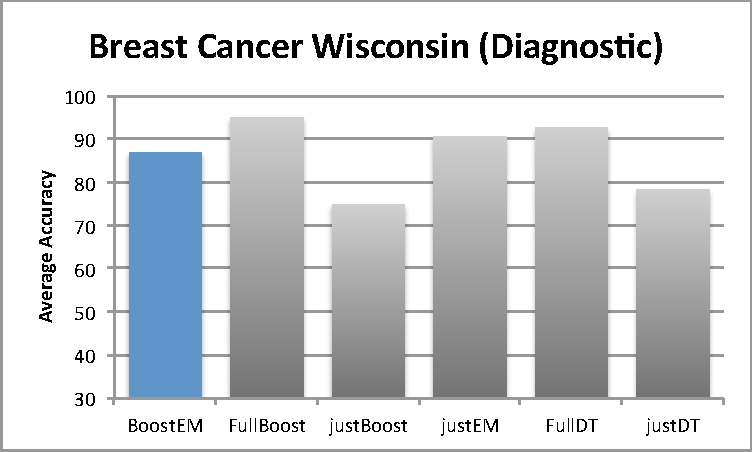
\includegraphics[width=0.3\textwidth]{figures/breaAcc5.pdf}
\caption{Average 10 fold cross validation \% accuracy using Naive Bayes on Various algorithms, 5\% labeled data}
\label{vertAcc}
\end{figure}

\section{Discussion}
STEVE 
\section{Conclusions}
%ACKNOWLEDGMENTS are optional
\section{Acknowledgments}

\bibliographystyle{abbrv}
\bibliography{paper}  % sigproc.bib is the name of the Bibliography in this case



\end{document}
